In this section we document the expected separatoins between 
the SM Higgs and spin 2 graviton hypothesis ($2_\text{min}^+$) calculated for \intlumiEightTeV 
at 8 TeV.  

Figure~\ref{fig:expsep} shows the distributions of 
$q=-2\text{ln}({\cal L}_{2_\text{min}^+}/{\cal L}_{\text{0}^+})$
with generated samples of background and signal of two types, 
SM $0^+$ and minimal couplings spin 2 $2_\text{min}^+$, for $m_H=$125 GeV. 
Here the likelihoods, $\cal L$, are calculated with the signal rates 
allowed to float indepdently for each signal type and the nusiance 
parameters are treated as independent. 
The expected distributions are generated with the same number of events 
after the full event selections. 
The mean of the expected SM $0^+$ distribution is 1.5 standard deviations 
in the tail of the $2_\text{min}^+$ distribution, while 
the mean of the expected $2_\text{min}^+$ distribution is 1.2 standard deviations 
in the tail of the $0^+$ distribution. 
The average separation between the two hypothesis is about $1.3\sigma$. 
The signal to background significance expected on average 
for the SM Higgs hypothesis is $3.3\sigma$, while for the spin 2 graviton $2_\text{min}^+$ 
model it is around $2.6\sigma$. 
%Scaling purely by luminosity, 
The expected average separation between the SM Higgs and $2_\text{min}^+$ 
hypotheses is about $1.7\sigma$ for 30~$\ifb$ scaling purely by luminosity. 


%%%%%%%%%%%%%%%%%%%%%%%%%%%%%%%%%%%%%%%%%%%%%
\begin{figure}[!hbtp]
\centering
\label{subfig:res}
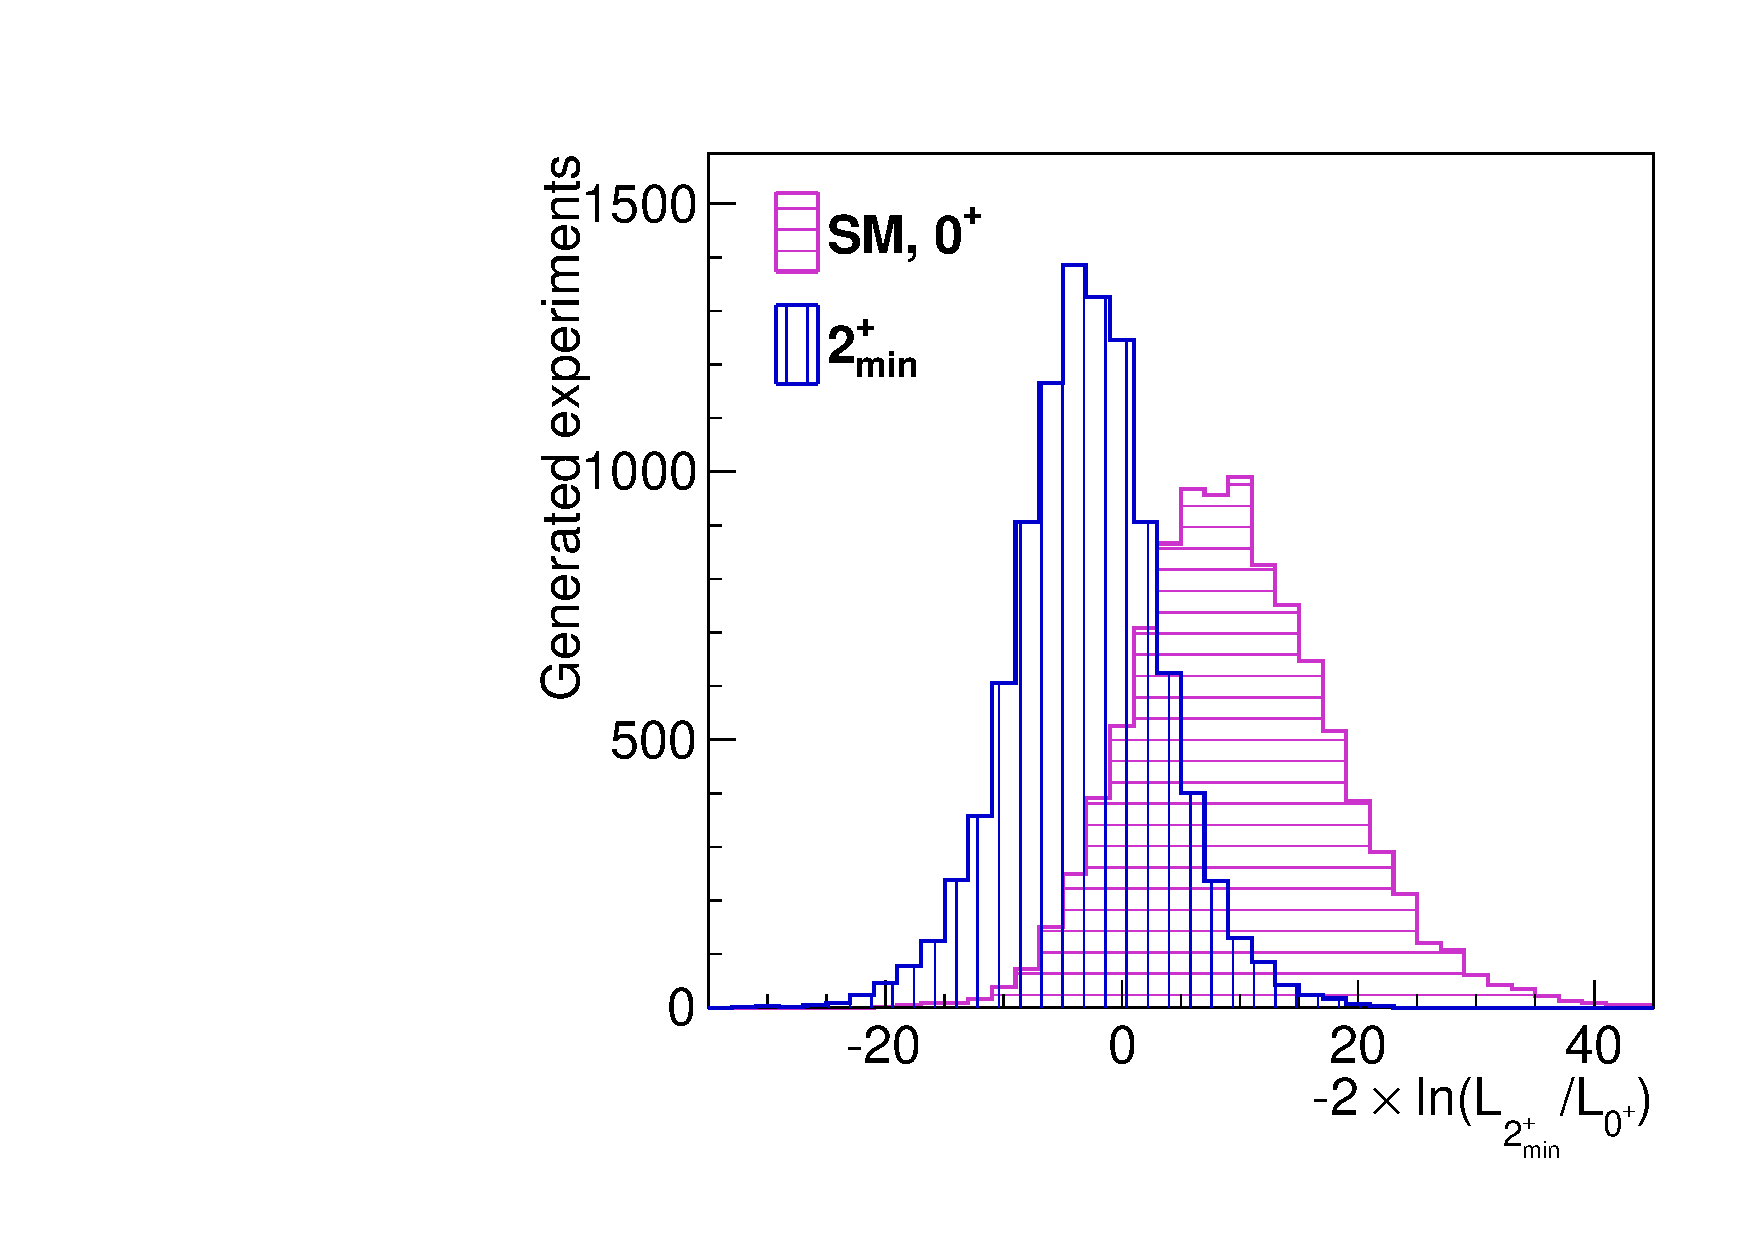
\includegraphics[width=.7\textwidth]{figures/hypo_separation.pdf}
\caption{Distributions of 
$q=-2\text{ln}({\cal L}_{2_\text{min}^+}/{\cal L}_{\text{0}^+})$, 
for two signal types ($0^+$ horizontally hatched histogram, 
$2_\text{min}^+$ vertically hatched histogram) for $m_H=$125 GeV. 
In these distributions 50K pseudo-datasets are generated for 
both hypotheses. }
\label{fig:expsep}
\end{figure}
%%%%%%%%%%%%%%%%%%%%%%%%%%%%%%%%%%%%%%%%%%%%%

